\documentclass[10pt,a4paper]{article}
\usepackage[utf8]{inputenc}
\usepackage{amsmath}
\usepackage{amsfonts}
\usepackage{amssymb}
\usepackage{graphicx}% Include figure files
\usepackage{bm}% bold math
\usepackage{color}
\usepackage[textsize=small]{todonotes}

\usepackage[top=1in, bottom=1in, left=1in, right=1in]{geometry}

\begin{document}
%%%%%%%%%%%%%%%%%%%%%%%%%%%%%%%%%%%%%%%%%%%%%%%%%%%%%%%%%%%%%%%%%%%%%%%%%%%%%%%
%\vspace*{\stretch{1.0}}
\begin{center}
\Large\textbf{Report 2: Bayesian learning in neural networks}\\
\large Author: \textit{Jannes Nys}
\end{center}
%\vspace*{\stretch{2.0}}
%%%%%%%%%%%%%%%%%%%%%%%%%%%%%%%%%%%%%%%%%%%%%%%%%%%%%%%%%%%%%%%%%%%%%%%%%%%%%%%

In this report, I discuss how Bayesian learning can be used as a method to avoid overfitting. Overfitting noisy data in the data set of Exercise session 1 occurs when the resulted fit shows large gradients in order to reproduce every single data points (which minimizes the cost function). However, the principle of Occam's razor dictates that overcomplex systems should be avoided for simple problems. When complexity rises, errors on the test set might increase, indicating overfitting. 

\section{`Pure' Bayesian training versus `trainbr'}
In the \texttt{perbayes} script, the weight values correspond the the MAP, i.e.\ the maximum of the posterior
\begin{equation}
\log P(\vec{w} | \mathcal{D}) = \log P(\mathcal{D} | \vec{w}) + \log P(\vec{w}) - \log P(\mathcal{D}) \,.
\end{equation}
for the data $\mathcal{D}$. Since the last term does not depend on the weight vector $\vec{w}$, we do not consider it in the following. Note that, if one compares this with the cost function $M$ in the assignment, we note that no hyper-parameters $\alpha$ and $\beta$ are included here. Therefore, we refer to this as the `pure' Bayesian algorithm. This is a restriction compared to the more general \texttt{trainbr} algorithm discussed below.\\

In order to understand the need for the hyper parameters, we vary the number of data points in the data set. For a high number of data points, the influence of the prior on the posterior is negligible. However, the likelihood calculates the probability of generating a set of discrete values ($0$ and $1$), from a continuous distribution (a sigmoid in this case). Naturally, the optimization converges to a sigmoid function which is as sharp as possible, corresponding to a weight vector in the outskirts of its domain. In the limit of an infinite data set, the modulus of the weight vector is over estimated, and the direction is incorrect. The latter is due to the fact that the modulus of the weight vector is largest when $|\vec{w}| = \sqrt{2}$. Hence, a sharp boundary is favoured over a correctly aligned boundary. In the case at hand, overfitting of the network corresponds to an overestimated $|\vec{w}|$. This effect we wish to counteract by introduction of the prior, wish gives a higher prior probability of obtaining smaller values of $|\vec{w}|$.

For similar reasons, the MAP does not always result in a weight vector which is close to the weight vector of the original network. In most cases, the weight vector has an over estimated modulus\footnote{For these reasons, angles of $45$, $135$ and $225$ and $315$ degrees are favoured. However, this effect is smaller for a lower number of data points.}. An example is shown in Fig~\ref{fig:example_perbayes}. Adjusting the effect of the prior properly can reduce this effect. Hence, introducing hyper parameters to scale the effect of the data and prior can improve the fitting. This is the case for the Bayesian regularization algorithm \texttt{trainbr}.
\begin{figure}[htb]
\centering
\begin{minipage}{0.2\textwidth}
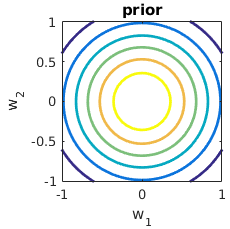
\includegraphics[height=2.5cm]{figs/prior_contour.png}
\end{minipage}%
\begin{minipage}{0.2\textwidth}
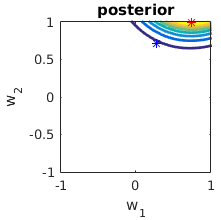
\includegraphics[height=2.5cm]{figs/posterior_contour.png}
\end{minipage}%
\begin{minipage}{0.2\textwidth}
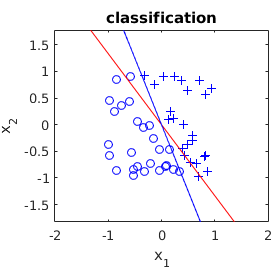
\includegraphics[height=2.5cm]{figs/separation_line.png}
\end{minipage}%
\caption{Prior, posterior and classification with corresponding separation line of the original (blue) and MAP network (red). Some (but not many) samples are misclassified.\label{fig:example_perbayes}}
\end{figure}

\section{Bayesian regularization using `trainbr'}
We now focus on the data set used in the previous report to discuss overfitting, and how Bayesian regulation my help reduce it.  An example of the effect of a Bayesian regularization term is illustrated in Fig.~\ref{fig:overfitting_example} where we compare the Maximum-a-posteriori result with a Maximum-Likelihood result.
\begin{figure}[htb]
\centering
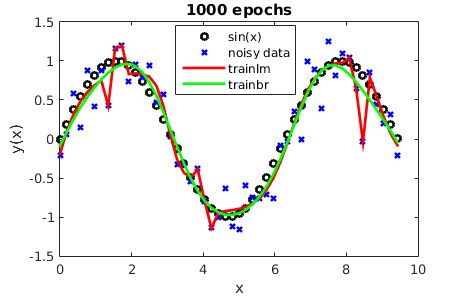
\includegraphics[width=0.5\textwidth]{figs/overfitting_example.png}
\caption{Illustration of an overfitted network trained with the Levenberg-Marquadt algorithm (red), compared to the results of the Bayesian learning (green) for a data set with $h(x)=\sin(x) + \mathcal{N}(\sigma)$ where $\sigma = 0.3$. Both networks have the same architecture, which includes $10$ neurons in the hidden layer.\label{fig:overfitting_example}}
\end{figure}
In the case at hand, in essence, we wish to approximate the underlying function $\sin(x)$ of the data, rather than the data set itself. In the Bayesian framework, regularization can be implemented in a natural way by opting for a parameter prior which has the bulk of its probability close to small values of the network weights. 

In the last report we characterized generalization and overfitting via the network's variance\footnote{Naturally, we could have also done this using a test set.}. We can therefore use the figure used in the previous report, now shown in Fig.~\ref{fig:bias_and_variance_plot}, and compare the \texttt{trainbr} algorithm with the other training algorithms. Figure~\ref{fig:bias_and_variance_plot} compares the bias and variance as a function of the complexity of the network for different learning algorithms.
 
\begin{figure}[hbt]
\centering
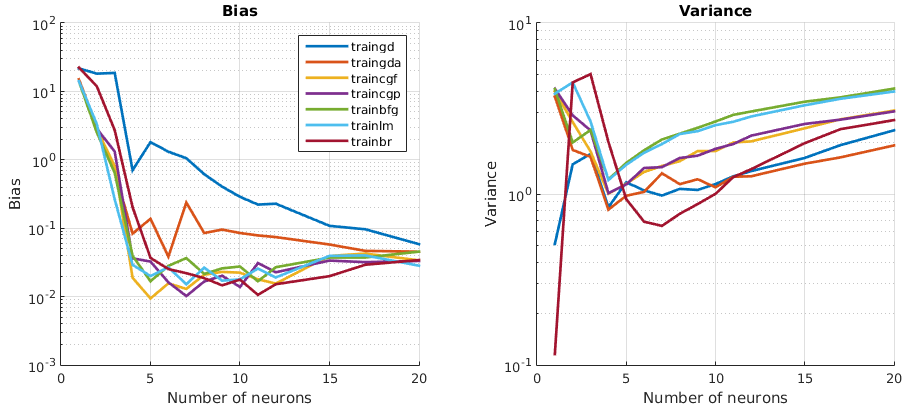
\includegraphics[width=\textwidth]{figs/bias_and_variance.png}
\caption{Bias and variance plot as a function of the complexity of the neural network.\label{fig:bias_and_variance_plot}}
\end{figure}

An overfitted network corresponds to a low bias but high variance in Fig.~\ref{fig:bias_and_variance_plot}. Assuming convergence has been reached, a large variance indicates that the resulting network depends largely on the data set to which it is fitted, and hence, to the noise it includes. The effect of the Bayesian regulation term is most clear in the interval of medium complexity (5-10 hidden neurons). Both the bias and variance remain low, indicating that the \texttt{trainbr} algorithm allows for a more accurate function reconstruction, while avoiding noise fitting (see again Fig.~\ref{fig:overfitting_example} for an illustration). Interestingly enough however, Fig.~\ref{fig:bias_and_variance_plot} also clearly shows the limited range of application of the Bayesian regulation. When the complexity is high enough, the regulation term has a negligible effect, and also \texttt{trainbr} will start overfitting.







\end{document}
